%        File: arfc-beamer.tex
%     Created: Sun May 5 10:00 PM 2013 C
%


%\documentclass[11pt,handout]{beamer}
\documentclass[9pt]{beamer}
\usetheme[white]{Illinois}
%\title[short title]{long title}
\title[Short Title]{Validation of Spent Nuclear Fuel Output by Cyclus, a Fuel Cycle Simulator Code}
%\subtitle[short subtitle]{long subtitle}
%\subtitle[Short SubTitle]{Mostly Kittens}
%\author[short name]{long name}
\author[Your Name]{Gwendolyn J. Chee, Gyutae Park \& Kathryn D. Huff \\ Advanced Reactors and Fuel Cycles Group}
%\date[short date]{long date}
\date[11.12.2018]{November 12, 2018}
%\institution[short name]{long name}
\institute[UIUC]{University of Illinois at Urbana-Champaign}

%\usepackage{bbding}
\usepackage{amsfonts}
\usepackage{amsmath}
\usepackage{xspace}
\usepackage{graphicx}
\usepackage{subfigure}
\usepackage{booktabs} % nice rules for tables
\usepackage{microtype} % if using PDF
\usepackage{bigints}
\usepackage{minted}

\newcommand{\units}[1] {\:\text{#1}}%
\newcommand{\SN}{S$_N$}%{S$_\text{N}$}%{$S_N$}%
\DeclareMathOperator{\erf}{erf}
%I need some complimentary error funcitons... 
\DeclareMathOperator{\erfc}{erfc}
%page numbers
\setbeamertemplate{footline}[page number]
\setbeamertemplate{caption}[numbered]
%Those icons in the references are terrible looking
\setbeamertemplate{bibliography item}[text]

%%%% Acronym support

\usepackage[acronym,toc]{glossaries}
%\newacronym{<++>}{<++>}{<++>}
\newacronym[longplural={metric tons of heavy metal}]{MTHM}{MTHM}{metric ton of heavy metal}
\newacronym{ABM}{ABM}{agent-based modeling}
\newacronym{ACDIS}{ACDIS}{Program in Arms Control \& Domestic and International Security}
\newacronym{AHTR}{AHTR}{Advanced High Temperature Reactor}
\newacronym{ANDRA}{ANDRA}{Agence Nationale pour la gestion des D\'echets RAdioactifs, the French National Agency for Radioactive Waste Management}
\newacronym{ANL}{ANL}{Argonne National Laboratory}
\newacronym{API}{API}{application programming interface}
\newacronym{ARE}{ARE}{Aircraft Reactor Experiment}
\newacronym{ARFC}{ARFC}{Advanced Reactors and Fuel Cycles}
\newacronym{ASME}{ASME}{American Society of Mechanical Engineers}
\newacronym{ATWS}{ATWS}{Anticipated Transient Without Scram}
\newacronym{BDBE}{BDBE}{Beyond Design Basis Event}
\newacronym{BIDS}{BIDS}{Berkeley Institute for Data Science}
\newacronym{CAFCA}{CAFCA}{ Code for Advanced Fuel Cycles Assessment }
\newacronym{CDTN}{CDTN}{Centro de Desenvolvimento da Tecnologia Nuclear}
\newacronym{CEA}{CEA}{Commissariat \`a l'\'Energie Atomique et aux \'Energies Alternatives}
\newacronym{CI}{CI}{continuous integration}
\newacronym{CNEN}{CNEN}{Comiss\~{a}o Nacional de Energia Nuclear}
\newacronym{CNERG}{CNERG}{Computational Nuclear Engineering Research Group}
\newacronym{COSI}{COSI}{Commelini-Sicard}
\newacronym{COTS}{COTS}{commercial, off-the-shelf}
\newacronym{CSNF}{CSNF}{commercial spent nuclear fuel}
\newacronym{CTAH}{CTAHs}{Coiled Tube Air Heaters}
\newacronym{CUBIT}{CUBIT}{CUBIT Geometry and Mesh Generation Toolkit}
\newacronym{CURIE}{CURIE}{Centralized Used Fuel Resource for Information Exchange}
\newacronym{DAG}{DAG}{directed acyclic graph}
\newacronym{DANESS}{DANESS}{Dynamic Analysis of Nuclear Energy System Strategies}
\newacronym{DBE}{DBE}{Design Basis Event}
\newacronym{DESAE}{DESAE}{Dynamic Analysis of Nuclear Energy Systems Strategies}
\newacronym{DHS}{DHS}{Department of Homeland Security}
\newacronym{DOE}{DOE}{Department of Energy}
\newacronym{DRACS}{DRACS}{Direct Reactor Auxiliary Cooling System}
\newacronym{DRE}{DRE}{dynamic resource exchange}
\newacronym{DSNF}{DSNF}{DOE spent nuclear fuel}
\newacronym{DYMOND}{DYMOND}{Dynamic Model of Nuclear Development }
\newacronym{EBS}{EBS}{Engineered Barrier System}
\newacronym{EDZ}{EDZ}{Excavation Disturbed Zone}
\newacronym{EIA}{EIA}{U.S. Energy Information Administration}
\newacronym{EPA}{EPA}{Environmental Protection Agency}
\newacronym{EP}{EP}{Engineering Physics}
\newacronym{FCO}{FCO}{Fuel Cycle Options}
\newacronym{FCT}{FCT}{Fuel Cycle Technology}
\newacronym{FEHM}{FEHM}{Finite Element Heat and Mass Transfer}
\newacronym{FEPs}{FEPs}{Features, Events, and Processes}
\newacronym{FHR}{FHR}{Fluoride-Salt-Cooled High-Temperature Reactor}
\newacronym{FLiBe}{FLiBe}{Fluoride-Lithium-Beryllium}
\newacronym{GDSE}{GDSE}{Generic Disposal System Environment}
\newacronym{GDSM}{GDSM}{Generic Disposal System Model}
\newacronym{GENIUSv1}{GENIUSv1}{Global Evaluation of Nuclear Infrastructure Utilization Scenarios, Version 1}
\newacronym{GENIUSv2}{GENIUSv2}{Global Evaluation of Nuclear Infrastructure Utilization Scenarios, Version 2}
\newacronym{GENIUS}{GENIUS}{Global Evaluation of Nuclear Infrastructure Utilization Scenarios}
\newacronym{GPAM}{GPAM}{Generic Performance Assessment Model}
\newacronym{GRSAC}{GRSAC}{Graphite Reactor Severe Accident Code}
\newacronym{GUI}{GUI}{graphical user interface}
\newacronym{HLW}{HLW}{high level waste}
\newacronym{HPC}{HPC}{high-performance computing}
\newacronym{HTC}{HTC}{high-throughput computing}
\newacronym{HTGR}{HTGR}{High Temperature Gas-Cooled Reactor}
\newacronym{IAEA}{IAEA}{International Atomic Energy Agency}
\newacronym{IEMA}{IEMA}{Illinois Emergency Mangament Agency}
\newacronym{INL}{INL}{Idaho National Laboratory}
\newacronym{IPRR1}{IRP-R1}{Instituto de Pesquisas Radioativas Reator 1}
\newacronym{IRP}{IRP}{Integrated Research Project}
\newacronym{ISFSI}{ISFSI}{Independent Spent Fuel Storage Installation}
\newacronym{ISRG}{ISRG}{Independent Student Research Group}
\newacronym{JFNK}{JFNK}{Jacobian-Free Newton Krylov}
\newacronym{LANL}{LANL}{Los Alamos National Laboratory}
\newacronym{LBNL}{LBNL}{Lawrence Berkeley National Laboratory}
\newacronym{LCOE}{LCOE}{levelized cost of electricity}
\newacronym{LDRD}{LDRD}{laboratory directed research and development}
\newacronym{LFR}{LFR}{Lead-Cooled Fast Reactor}
\newacronym{LLNL}{LLNL}{Lawrence Livermore National Laboratory}
\newacronym{LMFBR}{LMFBR}{Liquid Metal Fast Breeder Reactor}
\newacronym{LOFC}{LOFC}{Loss of Forced Cooling}
\newacronym{LOHS}{LOHS}{Loss of Heat Sink}
\newacronym{LOLA}{LOLA}{Loss of Large Area}
\newacronym{LP}{LP}{linear program}
\newacronym{MA}{MA}{minor actinide}
\newacronym{MCNP}{MCNP}{Monte Carlo N-Particle code}
\newacronym{MILP}{MILP}{mixed-integer linear program}
\newacronym{MIT}{MIT}{the Massachusetts Institute of Technology}
\newacronym{MOAB}{MOAB}{Mesh-Oriented datABase}
\newacronym{MOOSE}{MOOSE}{Multiphysics Object-Oriented Simulation Environment}
\newacronym{MOX}{MOX}{mixed oxide}
\newacronym{MSBR}{MSBR}{Molten Salt Breeder Reactor}
\newacronym{MSRE}{MSRE}{Molten Salt Reactor Experiment}
\newacronym{MSR}{MSR}{Molten Salt Reactor}
\newacronym{NAGRA}{NAGRA}{National Cooperative for the Disposal of Radioactive Waste}
\newacronym{NEAMS}{NEAMS}{Nuclear Engineering Advanced Modeling and Simulation}
\newacronym{NEUP}{NEUP}{Nuclear Energy University Programs}
\newacronym{NFCSim}{NFCSim}{Nuclear Fuel Cycle Simulator}
\newacronym{NGNP}{NGNP}{Next Generation Nuclear Plant}
\newacronym{NMWPC}{NMWPC}{Nuclear MW Per Capita}
\newacronym{NNSA}{NNSA}{National Nuclear Security Administration}
\newacronym{NPRE}{NPRE}{Department of Nuclear, Plasma, and Radiological Engineering}
\newacronym{NQA1}{NQA-1}{Nuclear Quality Assurance - 1}
\newacronym{NRC}{NRC}{Nuclear Regulatory Commission}
\newacronym{NSF}{NSF}{National Science Foundation}
\newacronym{NSSC}{NSSC}{Nuclear Science and Security Consortium}
\newacronym{NUWASTE}{NUWASTE}{Nuclear Waste Assessment System for Technical Evaluation}
\newacronym{NWF}{NWF}{Nuclear Waste Fund}
\newacronym{NWTRB}{NWTRB}{Nuclear Waste Technical Review Board}
\newacronym{OCRWM}{OCRWM}{Office of Civilian Radioactive Waste Management}
\newacronym{ORION}{ORION}{ORION}
\newacronym{ORNL}{ORNL}{Oak Ridge National Laboratory}
\newacronym{PARCS}{PARCS}{Purdue Advanced Reactor Core Simulator}
\newacronym{PBAHTR}{PB-AHTR}{Pebble Bed Advanced High Temperature Reactor}
\newacronym{PBFHR}{PB-FHR}{Pebble-Bed Fluoride-Salt-Cooled High-Temperature Reactor}
\newacronym{PEI}{PEI}{Peak Environmental Impact}
\newacronym{PH}{PRONGHORN}{PRONGHORN}
\newacronym{PRKE}{PRKE}{Point Reactor Kinetics Equations}
\newacronym{PSPG}{PSPG}{Pressure-Stabilizing/Petrov-Galerkin}
\newacronym{PWAR}{PWAR}{Pratt and Whitney Aircraft Reactor}
\newacronym{PWR}{PWR}{Pressurized Water Reactor}
\newacronym{PyNE}{PyNE}{Python toolkit for Nuclear Engineering}
\newacronym{PyRK}{PyRK}{Python for Reactor Kinetics}
\newacronym{QA}{QA}{quality assurance}
\newacronym{RDD}{RD\&D}{Research Development and Demonstration}
\newacronym{RD}{R\&D}{Research and Development}
\newacronym{RELAP}{RELAP}{Reactor Excursion and Leak Analysis Program}
\newacronym{RIA}{RIA}{Reactivity Insertion Accident}
\newacronym{RIF}{RIF}{Region-Institution-Facility}
\newacronym{SFR}{SFR}{Sodium-Cooled Fast Reactor}
\newacronym{SINDAG}{SINDA{\textbackslash}G}{Systems Improved Numerical Differencing Analyzer $\backslash$ Gaski}
\newacronym{SKB}{SKB}{Svensk K\"{a}rnbr\"{a}nslehantering AB}
\newacronym{SNF}{SNF}{spent nuclear fuel}
\newacronym{SNL}{SNL}{Sandia National Laboratory}
\newacronym{STC}{STC}{specific temperature change}
\newacronym{SUPG}{SUPG}{Streamline-Upwind/Petrov-Galerkin}
\newacronym{SWF}{SWF}{Separations and Waste Forms}
\newacronym{SWU}{SWU}{Separative Work Unit}
\newacronym{TRIGA}{TRIGA}{Training Research Isotope General Atomic}
\newacronym{TRISO}{TRISO}{Tristructural Isotropic}
\newacronym{TSM}{TSM}{Total System Model}
\newacronym{TSPA}{TSPA}{Total System Performance Assessment for the Yucca Mountain License Application}
\newacronym{ThOX}{ThOX}{thorium oxide}
\newacronym{UFD}{UFD}{Used Fuel Disposition}
\newacronym{UML}{UML}{Unified Modeling Language}
\newacronym{UOX}{UOX}{uranium oxide}
\newacronym{UQ}{UQ}{uncertainty quantification}
\newacronym{US}{US}{United States}
\newacronym{UW}{UW}{University of Wisconsin}
\newacronym{VISION}{VISION}{the Verifiable Fuel Cycle Simulation Model}
\newacronym{VV}{V\&V}{verification and validation}
\newacronym{WIPP}{WIPP}{Waste Isolation Pilot Plant}
\newacronym{YMR}{YMR}{Yucca Mountain Repository Site}


\makeglossaries

%try to get rid of header on title page\dots
\makeatletter
    \newenvironment{withoutheadline}{
        \setbeamertemplate{headline}[default]
        \def\beamer@entrycode{\vspace*{-\headheight}}
    }{}
\makeatother

\begin{document}
%%%%%%%%%%%%%%%%%%%%%%%%%%%%%%%%%%%%%%%%%%%%%%%%%%%%%%%%%%%%%
%% From uw-beamer Here's a handy bit of code to place at 
%% the beginning of your presentation (after \begin{document}):
\newcommand*{\alphabet}{ABCDEFGHIJKLMNOPQRSTUVWXYZabcdefghijklmnopqrstuvwxyz}
\newlength{\highlightheight}
\newlength{\highlightdepth}
\newlength{\highlightmargin}
\setlength{\highlightmargin}{2pt}
\settoheight{\highlightheight}{\alphabet}
\settodepth{\highlightdepth}{\alphabet}
\addtolength{\highlightheight}{\highlightmargin}
\addtolength{\highlightdepth}{\highlightmargin}
\addtolength{\highlightheight}{\highlightdepth}
\newcommand*{\Highlight}{\rlap{\textcolor{HighlightBackground}{\rule[-\highlightdepth]{\linewidth}{\highlightheight}}}}
%%%%%%%%%%%%%%%%%%%%%%%%%%%%%%%%%%%%%%%%%%%%%%%%%%%%%%%%%%%%%
%%--------------------------------%%
\begin{withoutheadline}
\frame{
  \titlepage
}
\end{withoutheadline}

%%--------------------------------%%
\AtBeginSection[]{
\begin{frame}
  \frametitle{Outline}
  \tableofcontents[currentsection]
\end{frame}
}

\section{Background and Motivation}
\subsection{Nuclear Waste Repository Model}
\begin{frame}
    \frametitle{Nuclear Waste Repository Model}
        \textbf{Long Term Goal}
        \\

        Run simulations to determine how varying certain variables in the nuclear fuel cycle impacts the mass loading of a nuclear waste repository for the U.S. nuclear fuel cycle. 
        \\

        Variables 
        \begin{itemize}
            \item used fuel allocation strategies
            \item waste package material properties 
            \item repository parameters
            \item presence of interim facilities
        \end{itemize}
\end{frame}
  
\subsection{Cyclus}
\begin{frame}
    \frametitle{Cyclus}
        \texttt{Cyclus} is an agent-based nuclear fuel cycle simulator with a modular architecture.
     \\   
    \begin{figure}[htbp!]
      \begin{center}
        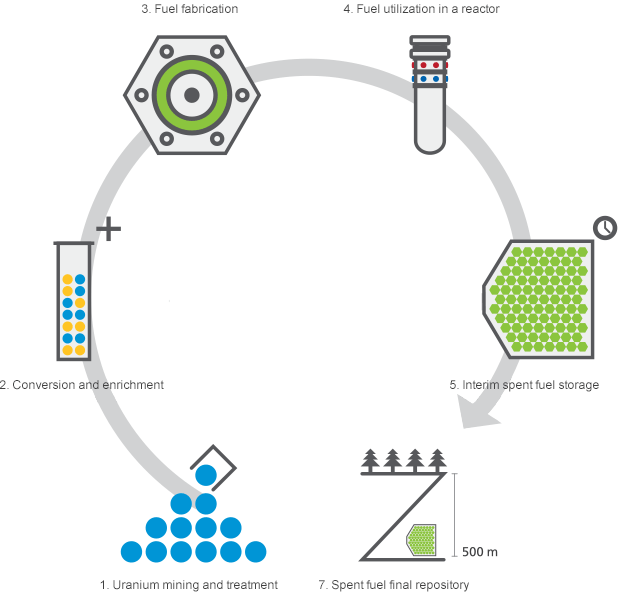
\includegraphics[height=5.3cm]{../figures/nfc}
      \end{center}
            \caption{Once Through Nuclear Fuel Cycle \cite{noauthor_nuclear_nodate}}
      \label{fig:cyclus-modular}
    \end{figure}
  \end{frame}
  
\subsection{Validation}
\begin{frame}
    \frametitle{Motivation for conducting the Validation}
    Waste package thermal evolution depends on the \textbf{decay heat contribution from each isotope} in the spent fuel. 
    \\
    
    Therefore, to \textbf{correctly simulate loading of a nuclear waste repository based on thermal constraints} in \textsc{Cyclus}, the simulation must first give isotopic compositions and spent fuel masses that \textbf{closely replicate reality}. 

  \end{frame}
  

\section{Method}
\subsection{Cyclus Simulation of historic U.S. nuclear fuel cycle}
\begin{frame}
    \frametitle{Cyclus Simulation of historic U.S. nuclear fuel cycle}
        Reactor deployment data obtained from the Power Reactor Information System (PRIS) database \cite{peterson_unf_2017} for the 112 commercial nuclear reactors that have operated since 1968 was used to create a \textsc{Cyclus} \textbf{simulation of the U.S. nuclear fuel cycle}. 
        \begin{columns}
        \column[t]{5cm}
    \begin{figure}[htbp!]
      \begin{center}
        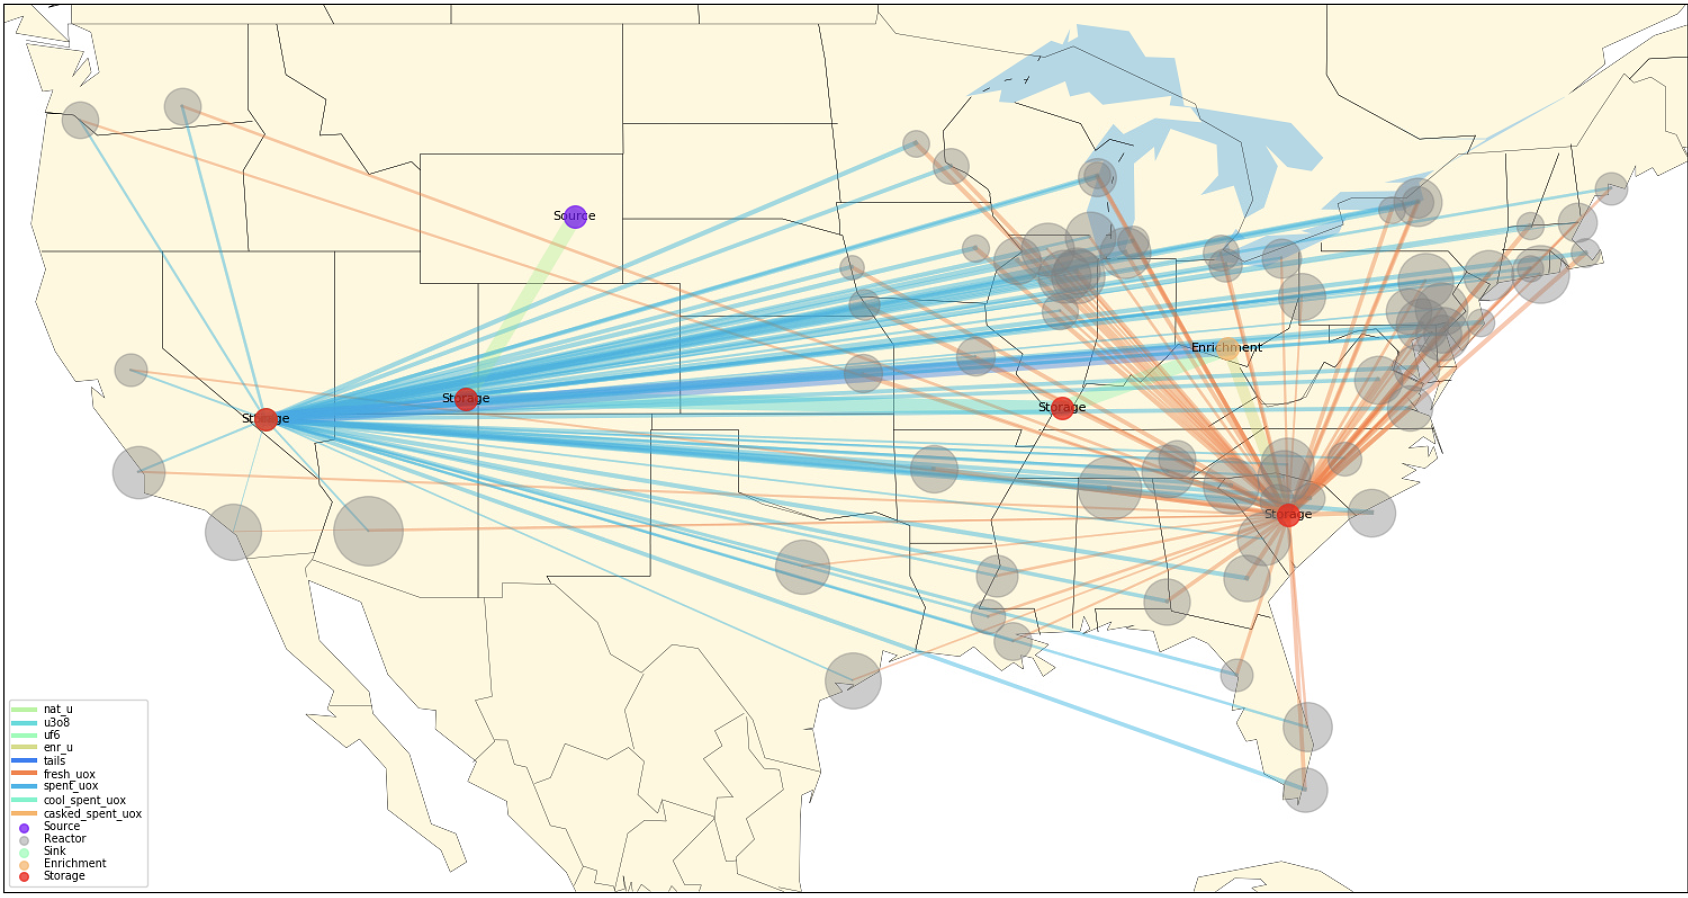
\includegraphics[height=3cm]{../figures/cycmap}
      \end{center}
            \caption{Cycmap of the historic Cyclus U.S nuclear fuel cycle simulation \cite{park_arfc/cycmap_2018}}
      \label{fig:cycmap}
    \end{figure}
    \column[t]{5cm}
    \textbf{Assumptions} 
    \begin{itemize}
    \item constant refueling time 
    \item constant reactor cycle time 
    \item single spent fuel depletion composition
    \end{itemize}
  \end{columns}
  \end{frame}

\subsection{Comparison of Cyclus Simulation against Unified Database}
\begin{frame}
    \frametitle{Comparison of Cyclus Simulation against Unified Database}
    The total spent fuel mass and specific isotopic compositions from the \textsc{Cyclus} 
        simulation and Unified Database were \textbf{compared}. 
        \\ 
        
    Unified Database is part of a larger engineering analysis tool, the Used Nuclear Fuel Storage, 
    Transportation \& Disposal Analysis Resource and Data System (UNF-ST\&DARDS). 
    \\

    It contains \textbf{commercial SNF information} from 1968 through 2013. \cite{peterson_unf_2017}. 
        \\ 
        
        \begin{figure}[htbp!]
            \begin{center}
                
\includegraphics[height=2.5cm]{../figures/peterson-unf}
            \end{center}
                    \caption{UNF-ST\&ARDS Unified Database and the Automatic
                    Document Generator Journal Article}
            \label{fig:peterson-unf}
            \end{figure}
\end{frame}
  
\section{Results}
\subsection{Cyclus vs. Unified Database: Total Spent Fuel Mass}
\begin{frame}
    \frametitle{Cyclus vs. Unified Database: Total Spent Fuel Mass}
       
    \begin{figure}[htbp!]
      \begin{center}
        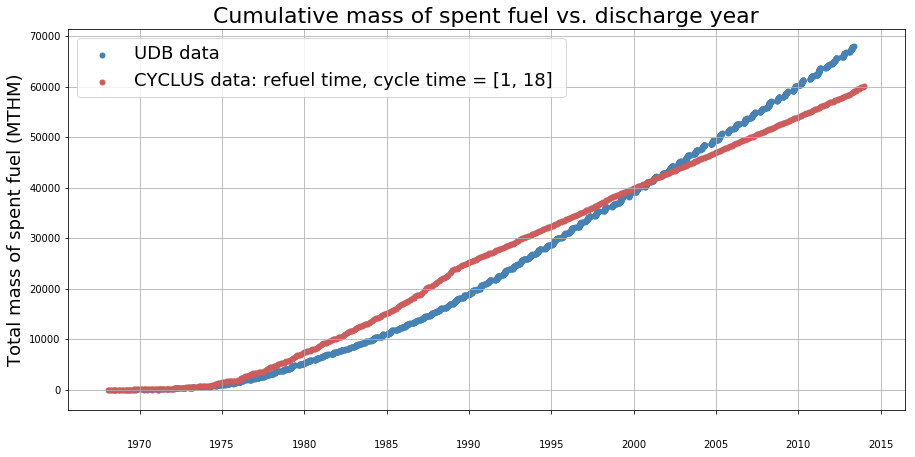
\includegraphics[height=5cm]{../figures/cumulative_mass_udb_cyclus}
      \end{center}
            \caption{The cumulative spent fuel mass against discharge time
            for Cyclus and Unified Database data from 1968 through 2013.}
      \label{fig:totalmass}
    \end{figure}
  \end{frame}

\begin{frame}
    \frametitle{Varying Refueling and Cycle durations in Cyclus Simulation}
    \begin{figure}[htbp!]
        \begin{center}
        \subfigure{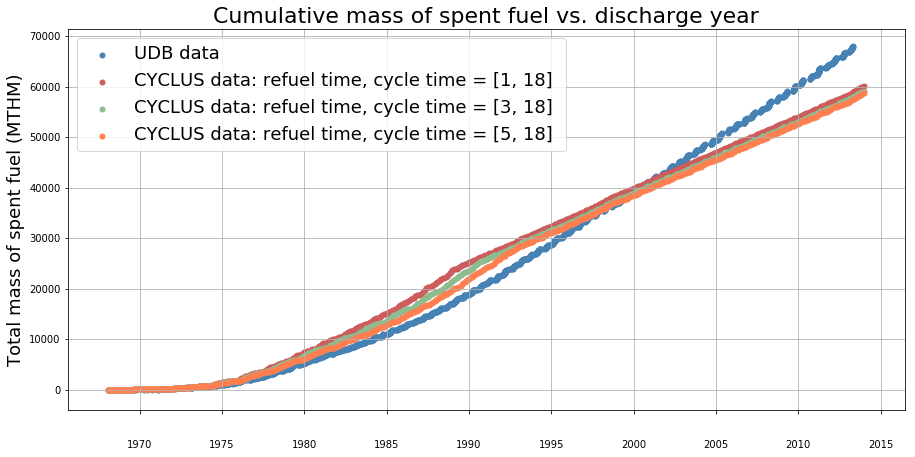
\includegraphics[height=2.8cm]{../figures/cumulative_mass_udb_cyclus_refueltime}}
        \subfigure{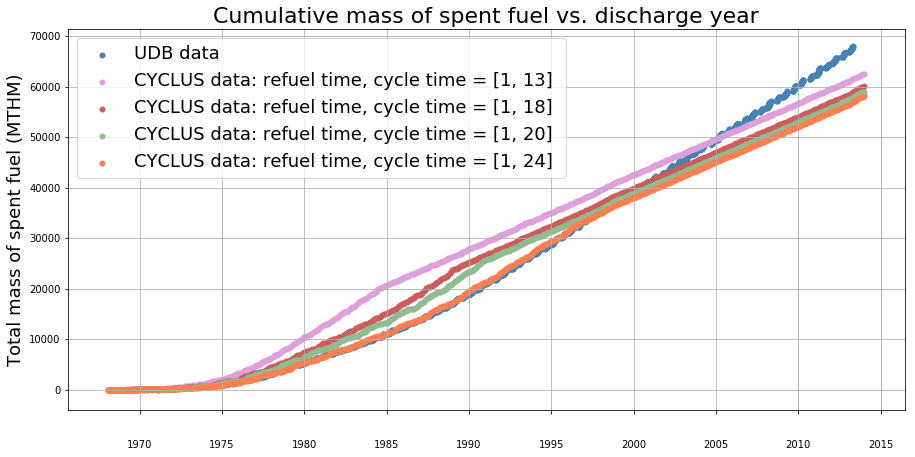
\includegraphics[height=2.8cm]{../figures/cumulative_mass_udb_cyclus_cycletime}}
        \end{center}
        \caption{The cumulative spent fuel mass against discharge time
        for Cyclus and Unified Database data from 1968 through 2013 for varying
        \textbf{refueling and cycle durations}.}
    \end{figure}  
\end{frame}
\subsection{Cyclus vs. Unified Database: Major Isotopic Composition}
\begin{frame}
    \frametitle{Cyclus vs. Unified Database: Major Isotopic Composition}
    \begin{figure}[htbp!]
        \begin{center}
          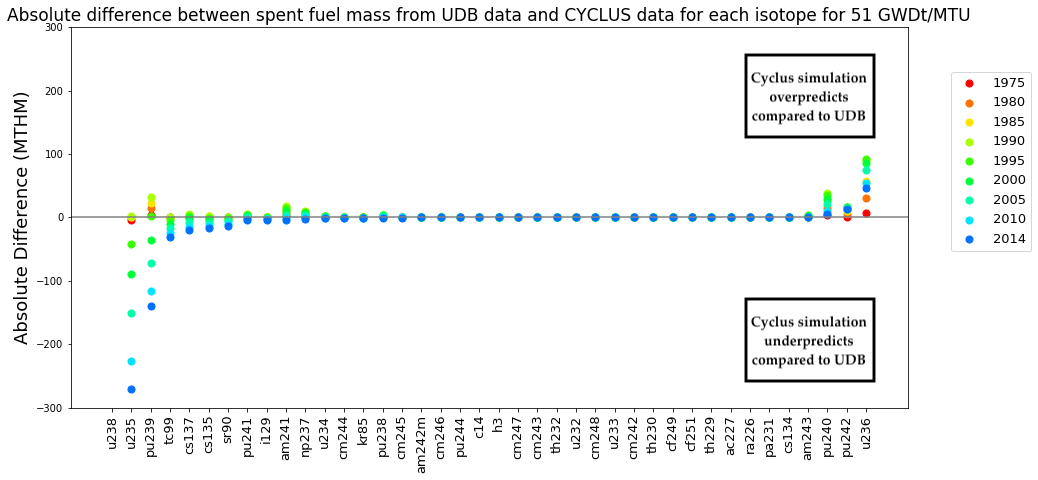
\includegraphics[height=5.3cm]{../figures/absolute_diff_all_51}
        \end{center}
              \caption{The absolute difference between cumulative spent fuel mass calculated by 
              Unified Database and \textsc{Cyclus} for each isotope. Spent fuel burnup of 51 GWD/MTU is used in the \textsc{Cyclus} simulation.
              Positive difference indicates \textsc{Cyclus}
              mass estimate is larger.}
        \label{fig:totalmass}
      \end{figure}
\end{frame}

\begin{frame}
    \frametitle{Cyclus vs. Unified Database: Major Isotopic Composition}
    \begin{figure}[htbp!]
        \begin{center}
          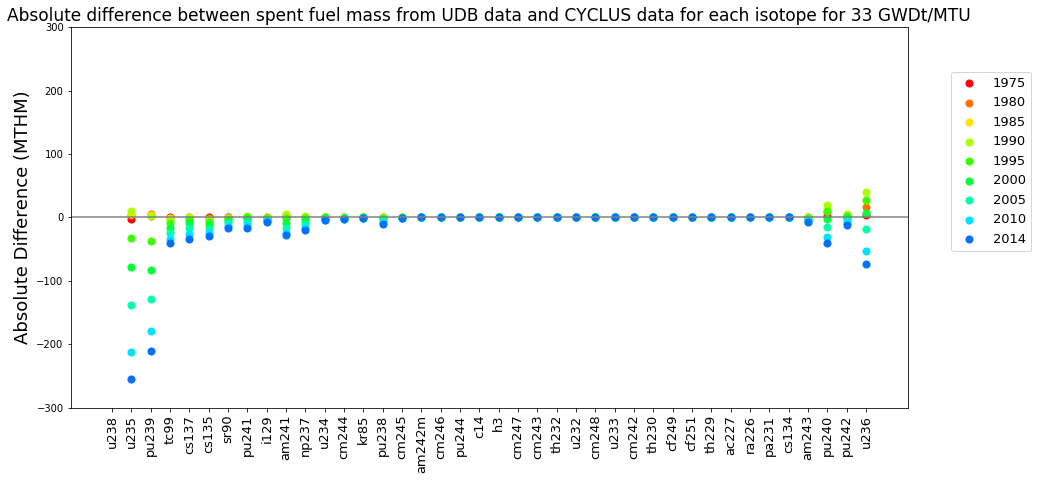
\includegraphics[height=5.3cm]{../figures/absolute_diff_all_33}
        \end{center}
        \caption{The absolute difference between cumulative spent fuel mass calculated by 
        Unified Database and \textsc{Cyclus} for each isotope. Spent fuel burnup of 33 GWD/MTU is used in the \textsc{Cyclus} simulation.
        Positive difference indicates \textsc{Cyclus}
        mass estimate is larger.}
        \label{fig:totalmass}
      \end{figure}
\end{frame}

\begin{frame}
    \frametitle{Burn up of Spent Nuclear Fuel}
    \begin{columns}
        \column[t]{5cm}
        \begin{figure}[htbp!]
        \begin{center}
        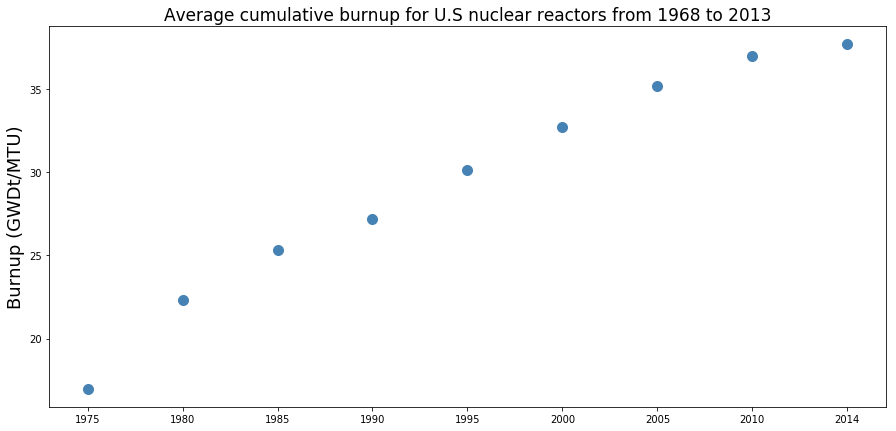
\includegraphics[height=2.8cm]{../figures/burn_up_real}
        \end{center}
        \caption{The average cumulative burnup for U.S. nuclear reactors
        from 1968 to 2013 \cite{eia_spent_2015}.}
        \end{figure}
        \column[t]{5cm}
        \begin{figure}[htbp!]
            \begin{center}
            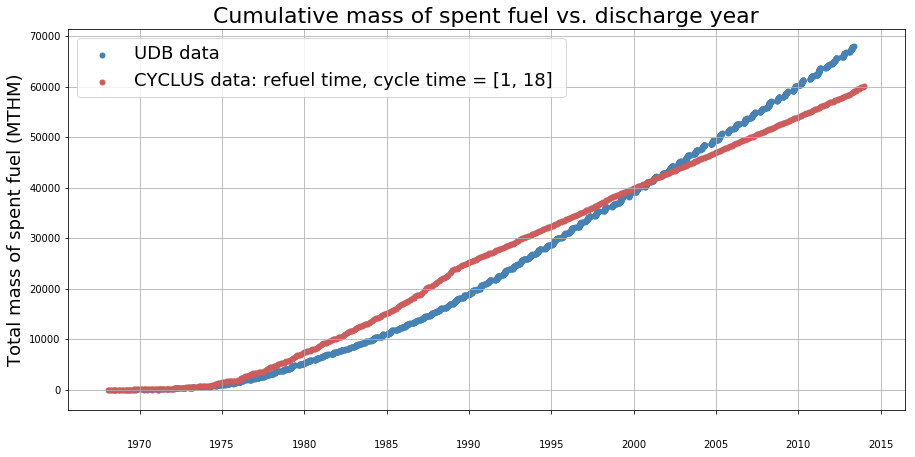
\includegraphics[height=2.8cm]{../figures/cumulative_mass_udb_cyclus}
            \end{center}
                \caption{The cumulative spent fuel mass against discharge time
                for Cyclus and Unified Database data from 1968 through 2013.}
          \label{fig:totalmass}
            \end{figure}
    \end{columns}
\end{frame}

\begin{frame}
    \frametitle{Cyclus vs. Unified Database: Major Isotopic Composition}
    \begin{figure}[htbp!]
        \begin{center}
          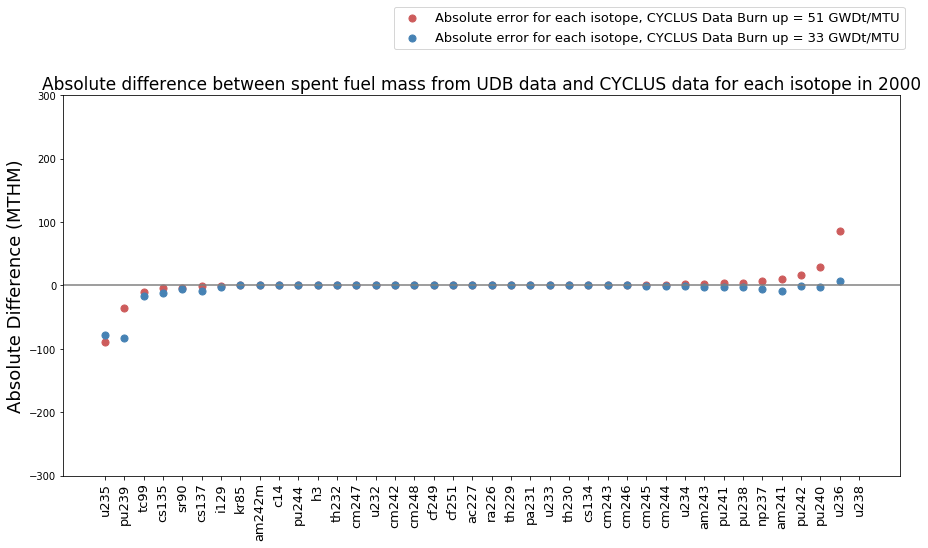
\includegraphics[height=6cm]{../figures/absolute_diff_2000}
        \end{center}
              \caption{The absolute difference between cumulative spent fuel mass calculated by 
              Unified Database and \textsc{Cyclus} for each isotope at year 2000. Positive difference indicates \textsc{Cyclus}
              mass estimate is larger.}
        \label{fig:totalmass}
      \end{figure}
\end{frame}

\begin{frame}
    \frametitle{Cyclus vs. Unified Database: Major Isotopic Composition}
    \begin{figure}[htbp!]
        \begin{center}
          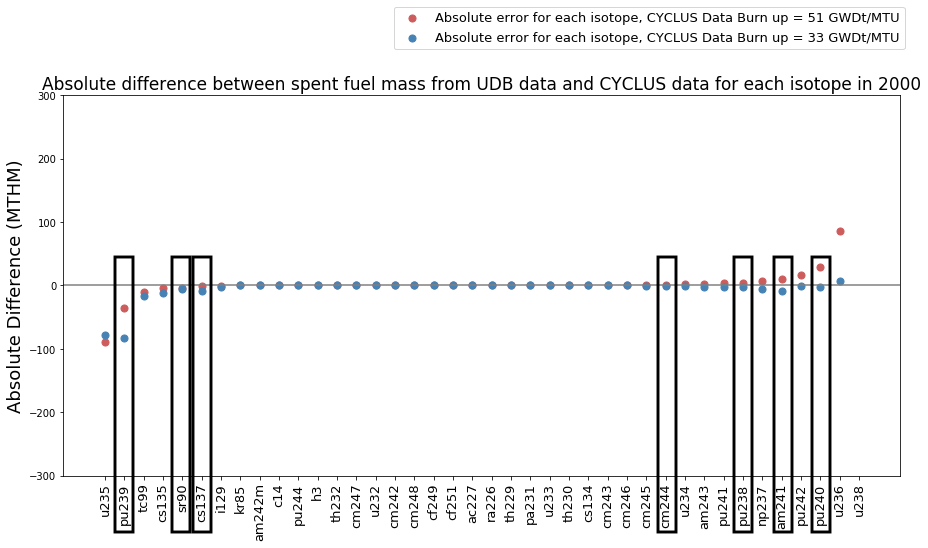
\includegraphics[height=6cm]{../figures/absolute_diff_2000_annotated}
        \end{center}
              \caption{The absolute difference between cumulative spent fuel mass calculated by 
              Unified Database and \textsc{Cyclus} for each isotope at year 2000. The boxed isotopes are the major decay heat contributors.}
        \label{fig:totalmass}
      \end{figure}
\end{frame}
\section{Conclusion}
\subsection{Conclusion}
\begin{frame}
  \frametitle{Conclusion}
        These results demonstrate that the spent fuel mass and isotopic
        composition calculated by the Cyclus simulation for
        the US nuclear fuel cycle follow \textbf{similar trends} as the real
        world metrics.
        \\
        
        Deviations from the real world metric can be explained by issues with 
        the reactor facility in the \textsc{Cyclus} model: 
        \begin{itemize}
                \item only accepting integer month values for
                cycle and refueling durations
                \item single spent fuel recipe 
        \end{itemize}
        
\end{frame}

\subsection{Future Work}
\begin{frame}
    \frametitle{Future Work}
          To more accurately model isotopic concentrations in the \textsc{Cyclus} simulation, 
          these capabilities could be implemented in \textsc{Cyclus}:
          \begin{itemize}
              \item Simple: Toolkit that ties the reactor facility to a database of varying spent fuel recipes based on burnup 
              \item Complex: Toolkit that ties the reactor facility to the UDB database to give different spent fuel recipes based on the burnup of a specific spent fuel bundle
              \item Toolkit that gives the functionality of varying cycle time and refuel duration values 
          \end{itemize} 
          
  \end{frame}
  
\begin{frame}
  \frametitle{Acknowledgement}
  This work is supported by U.S. Department of Energy, 
  Nuclear Energy University Program, under contract 
  \#NEUP-FY16-10512. 
  \end{frame}

%%--------------------------------%%
%%--------------------------------%%
\begin{frame}[allowframebreaks]
  \frametitle{References}
  \bibliographystyle{plain}
  {\footnotesize \bibliography{../docs/bibliography.bib} }

\end{frame}

%%--------------------------------%%


\end{document}



